\documentclass[aspectratio=169,10pt]{beamer}
\usetheme{Madrid}
\usecolortheme{default}
\usepackage{tikz}
\usepackage{booktabs}
\usepackage{fontawesome5}
\usepackage{xcolor}
\usepackage{amsmath}
\usepackage{colortbl}
\usepackage{multirow}
\usetikzlibrary{arrows.meta,shadows,positioning,fit,shapes.geometric,calc}

% ── palette ──────────────────────────────────────────────────────────
\definecolor{c1}{RGB}{41,128,185}
\definecolor{c2}{RGB}{52,152,219}
\definecolor{c3}{RGB}{155,89,182}
\definecolor{c4}{RGB}{142,68,173}
\definecolor{c5}{RGB}{230,126,34}
\definecolor{c6}{RGB}{211,84,0}
\definecolor{hit}{RGB}{39,174,96}
\definecolor{miss}{RGB}{192,57,43}
\definecolor{warn}{RGB}{243,156,18}

\setbeamercolor{frametitle}{bg=c1,fg=white}
\setbeamercolor{title}{fg=white}
\setbeamercolor{structure}{fg=c1}
\setbeamertemplate{navigation symbols}{}
\setbeamertemplate{footline}[frame number]
\setbeamerfont{frametitle}{series=\bfseries}

\newcommand{\chit}[1]{\cellcolor{hit!30} #1}
\newcommand{\cmiss}[1]{\cellcolor{miss!25} #1}
\newcommand{\cwarn}[1]{\cellcolor{warn!30} #1}
\newcommand{\czero}{\cellcolor{black!4} }

\title{\textbf{Graph-Based Vulnerability Retrieval}\\[4pt]}
\subtitle{Master's Thesis — Technical Progress · Checkpoint 6}
\author{Lívia}
\institute{TU Munich · Siemens}
\date{\today}


\begin{document}

% ── title ─────────────────────────────────────────────────────────────
\begin{frame}
\titlepage
\end{frame}

% ── agenda ────────────────────────────────────────────────────────────
% \begin{frame}{Agenda}
%   \begin{enumerate}
%     \item[\textcolor{c1}{\faIcon{database}}]
%       \textbf{CVEfixes Dataset Integration} — database extraction, statistics, and filtering

%     \vspace{0.45em}
%     \item[\textcolor{c3}{\faIcon{project-diagram}}]
%       \textbf{Preliminary CPG Study} — Joern graph generation on 10 diverse CVEs

%     \vspace{0.45em}
%     \item[\textcolor{c5}{\faIcon{cut}}]
%       \textbf{Slicing Depth Study} — comparing 6 slice configurations on CVEfixes

%     \vspace{0.45em}
%     \item[\textcolor{hit}{\faIcon{brain}}]
%       \textbf{GNN Triplet Training (CWE families)} — ReGVD with triplet loss on 695 graphs

%     \vspace{0.45em}
%     \item[\textcolor{c4}{\faIcon{crosshairs}}]
%       \textbf{Token-Guided Slicing \& Clustering} — discriminative token strategies

%     \vspace{0.45em}
%     \item[\textcolor{miss}{\faIcon{search}}]
%       \textbf{Joern Sink Verification} — pattern-based sink identification vs.\ ground truth
%   \end{enumerate}
% \end{frame}


% ══════════════════════════════════════════════════════════════════════
\section{CVEfixes Dataset Integration}
% ══════════════════════════════════════════════════════════════════════

\begin{frame}{CVEfixes Dataset Integration: Overview}
\begin{columns}[T]
\begin{column}{0.50\textwidth}

  \textbf{Goal}\\[3pt]
  {\small Integrate the CVEfixes database into our pipeline to
  obtain a large-scale knowledge base of historical vulnerability fixes.
  Verify that our CPG+embedding approach generalises beyond the 70-sample AutoPatch corpus.}

  \vspace{0.6em}
  \textbf{Database Scale}
  \begin{description}[\textbf{methods}]
    \item[\textbf{CVEs}] 11,873 vulnerabilities
    \item[\textbf{commits}] 12,107 fix commits
    \item[\textbf{files}] 51,342 changed files
    \item[\textbf{methods}] 277,948 method changes
  \end{description}

% ADD HERE 
      \textbf{Predominantly C code (92\%)} — consistent with kernel/system-level focus of our pipeline.
      Average patch adds 22 lines and removes 5 lines (asymmetric fixes).
\end{column}
\begin{column}{0.47\textwidth}

  \centering
  \vspace{0.5em}
  {\small\textbf{Extracted Corpus Statistics}}\\[6pt]
  {\scriptsize
  \renewcommand{\arraystretch}{1.25}
  \begin{tabular}{lr}
    \toprule
    \textbf{Metric} & \textbf{Value} \\
    \midrule
    Method pairs & 4,607 \\
    Unique CVEs & 1,777 \\
    Unique CWEs & 92 \\
    Languages & C (92\%), C++ (8\%) \\
    \midrule
    Avg lines added & 22.4 \\
    Avg lines removed & 5.4 \\
    Avg similarity ratio & 0.563 \\
    \midrule
    Severity: CRITICAL & 557 \\
    Severity: HIGH & 1,132 \\
    Severity: MEDIUM & 1,388 \\
    \bottomrule
  \end{tabular}}

\end{column}
\end{columns}
\end{frame}


\begin{frame}{CVEfixes: CWE Distribution \& Filtering}
\begin{columns}[T]
\begin{column}{0.48\textwidth}

  \textbf{Top CWEs in CVEFixes}\\[4pt]
  {\scriptsize
  \renewcommand{\arraystretch}{1.2}
  \begin{tabular}{llr}
    \toprule
    \textbf{CWE} & \textbf{Name} & \textbf{Count} \\
    \midrule
    CWE-119 & Buffer Overflow & 507 \\
    CWE-125 & Out-of-bounds Read & 393 \\
    CWE-20  & Improper Validation & 308 \\
    CWE-416 & Use After Free & 304 \\
    CWE-476 & NULL Ptr Deref & 259 \\
    CWE-362 & Race Condition & 250 \\
    CWE-787 & Out-of-bounds Write & 150 \\
    CWE-190 & Integer Overflow & 137 \\
    CWE-400 & Resource Exhaustion & 137 \\
    CWE-401 & Memory Leak & 77 \\
    \bottomrule
  \end{tabular}}

\end{column}
\begin{column}{0.50\textwidth}

  \textbf{AutoPatch CWE Overlap Filter}\\[4pt]
  {\small Filtered CVEfixes to CWEs present in the AutoPatch dataset
  (23 CWE types) to ensure the expanded corpus covers the same
  vulnerability families.}

  \vspace{0.5em}
  {\scriptsize
  \renewcommand{\arraystretch}{1.2}
  \begin{tabular}{lr}
    \toprule
    \textbf{Metric} & \textbf{Value} \\
    \midrule
    AutoPatch CWE types & 23 \\
    CVEfixes entries matching & \textbf{1,618} \\
    Coverage of extracted corpus & 35.1\% \\
    \midrule
    CVE-based filter (exact CVEs) & 0 \\
    \bottomrule
  \end{tabular}}

  \vspace{0.5em}
  {\small\textcolor{c1}{\faIcon{info-circle}} Zero CVE overlap — purely temporal:
  CVEfixes ends July 2024; AutoPatch CVEs are from late 2024--2025.
  The datasets are fully complementary (same CWE families, disjoint time periods).}

\end{column}
\end{columns}
\end{frame}


% \begin{frame}{CVEfixes: Key Findings}
%   \begin{enumerate}
%     \item[\textcolor{c1}{\faIcon{chart-bar}}]
%       \textbf{4,607 method pairs extracted} — 40$\times$ larger than AutoPatch corpus (70 samples),
%       enabling meaningful train/test splits for embedding evaluation.
%       \textit{CWE-filtered subset (1,618) is 23$\times$ larger.}

%     \vspace{0.3em}
%     \item[\textcolor{hit}{\faIcon{check-circle}}]
%       \textbf{Strong CWE overlap with AutoPatch} — 23 shared CWE types covering UAF, NPD,
%       race conditions, integer overflow, and resource leaks.
%       \textit{Same vulnerability families, different real-world instances.}

%     \vspace{0.3em}
%     \item[\textcolor{warn}{\faIcon{bug}}]
%       \textbf{No CVE-level overlap} — CVEfixes and AutoPatch fix different vulnerabilities entirely.
%       \textit{CVEfixes becomes our external knowledge base; AutoPatch remains the test set.}

%     \vspace{0.3em}
%     \item[\textcolor{c3}{\faIcon{code}}]
%       \textbf{Predominantly C code (92\%)} — consistent with kernel/system-level focus of our pipeline.
%       Average patch adds 22 lines and removes 5 lines (asymmetric fixes).
%   \end{enumerate}
% \end{frame}


% ══════════════════════════════════════════════════════════════════════
\section{Preliminary CPG Study}
% ══════════════════════════════════════════════════════════════════════

\begin{frame}{Preliminary CPG Study: Experiment Design}
\begin{columns}[T]
\begin{column}{0.50\textwidth}

  \textbf{Goal}\\[3pt]
  {\small Validate that our Joern CPG generation + graph-diff pipeline
  works on CVEfixes data. Question: does the diff-based slicing algorithm
  produce meaningful vulnerability subgraphs on this new dataset?}

  \vspace{0.6em}
  \textbf{Setup}
  \begin{description}[\textbf{Diversity}]
    \item[\textbf{N}] 10 examples, 10–50 lines each
    \item[\textbf{CWEs}] 190, 362, 125, 285, 20, 367, 1284, 401, 264, 416
    \item[\textbf{Pipeline}] Joern export $\to$ load CPG $\to$ compute\_graph\_diff
  \end{description}

\end{column}
\begin{column}{0.47\textwidth}

  \textbf{Key Result}\\[4pt]
  {\small\textcolor{hit}{\faIcon{check-circle}} 8/10 produce valid slices.
  Pipeline generalises to CVEfixes without modification.}

  \vspace{0.5em}
  {\small\textcolor{warn}{\faIcon{exclamation-triangle}} Slices are large
  (60--90\% of CPG). Fix-adjacent nodes dominate.}

  \vspace{0.5em}
  {\small\textcolor{miss}{\faIcon{times-circle}} 2/10 fail: very small functions
  (7 nodes) where Joern produces trivial graphs. These have no semantic content
  to slice.}
\end{column}
\end{columns}
\end{frame}


\begin{frame}{Preliminary CPG Study: Results}

  \centering
  \vspace{0.2em}
  {\scriptsize
  \renewcommand{\arraystretch}{1.3}
  \setlength{\tabcolsep}{3.5pt}
  \begin{tabular}{llrr|rrrr}
    \toprule
    & & \multicolumn{2}{c|}{\textit{nodes}} & \multicolumn{4}{c}{\textit{unique source lines}} \\
    \cmidrule(lr){3-4} \cmidrule(lr){5-8}
    \textbf{\#} & \textbf{CVE / CWE} & \textbf{Before} & \textbf{After}
      & \textbf{Slice} & \textbf{Removed} & \textbf{Fix-adj} & \textbf{GT} \\
    \midrule
    1 & CVE-2024-22862 / CWE-190 & 265 & 281 & 33 & 3 & 24 & 2 \\
    2 & CVE-2020-12652 / CWE-362 & 7 & 7 & 0 & 0 & 0 & 2 \\
    3 & CVE-2018-8789 / CWE-125  & 106 & 107 & 9 & 1 & 9 & 2 \\
    4 & CVE-2016-7097 / CWE-285  & 7 & 7 & 0 & 0 & 0 & 12 \\
    5 & CVE-2013-7271 / CWE-20   & 287 & 275 & 32 & 21 & 20 & 5 \\
    6 & CVE-2022-1974 / CWE-367  & 264 & 256 & 32 & 3 & 31 & 2 \\
    7 & CVE-2022-25375 / CWE-1284 & 194 & 231 & 22 & 17 & 7 & 3 \\
    8 & CVE-2019-19079 / CWE-401 & 151 & 160 & 15 & 6 & 12 & 5 \\
    9 & CVE-2016-3841 / CWE-264  & 284 & 302 & 29 & 11 & 24 & 5 \\
    10 & CVE-2017-16939 / CWE-416 & 202 & 121 & 17 & 14 & 7 & 8 \\
    \bottomrule
  \end{tabular}}

  \vspace{0.5em}
  \begin{columns}[T]
  \begin{column}{0.32\textwidth}
    {\scriptsize\textbf{\textcolor{hit}{Successes}}}
    \begin{itemize}\itemsep1pt
      {\scriptsize
      \item 8/10 produced non-empty slices
      \item Pipeline handles diverse CWEs}
    \end{itemize}
  \end{column}
  \begin{column}{0.32\textwidth}
    {\scriptsize\textbf{\textcolor{warn}{Observations}}}
    \begin{itemize}\itemsep1pt
      {\scriptsize
      \item Fix-adjacent nodes dominate slices
      \item Slices are 60–90\% of full CPG}
    \end{itemize}
  \end{column}
  \begin{column}{0.32\textwidth}
    {\scriptsize\textbf{\textcolor{miss}{Failures}}}
    \begin{itemize}\itemsep1pt
      {\scriptsize
      \item 2/10 produced empty slices (7 nodes)
      \item Small functions → Joern parse issues}
    \end{itemize}
  \end{column}
  \end{columns}
\end{frame}


% ══════════════════════════════════════════════════════════════════════
\section{Slicing Depth Study}
% ══════════════════════════════════════════════════════════════════════

\begin{frame}{Slicing Depth Study: Experiment Design}
\begin{columns}[T]
\begin{column}{0.50\textwidth}

  \textbf{Goal}\\[3pt]
  {\small The preliminary study showed slices are 60--90\% of the full CPG —
  too large, diluting the vulnerability signal. Question: how much
  flow context around changed nodes is actually needed?}

  \vspace{0.5em}
  \textbf{Metrics}
  \begin{description}[\textbf{CWE recall}]
    \item[\textbf{hit@K}] Query's CWE family in top-K retrieved results
    \item[\textbf{MRR}] Mean reciprocal rank of first same-CWE hit
    \item[\textbf{CWE recall}] Fraction of CWE families covered in top-K
  \end{description}

  \vspace{0.5em}
  \textbf{Hypothesis}\\[3pt]
  {\small Tighter slices (fewer context nodes) should improve embedder
  discrimination by concentrating the change signal.}

\end{column}
\begin{column}{0.47\textwidth}

  {\small\textbf{Slice Configurations}}\\[4pt]
  {\scriptsize
  \renewcommand{\arraystretch}{1.25}
  \begin{tabular}{p{2.2cm}p{1.0cm}p{2.2cm}}
    \toprule
    \textbf{Config} & \textbf{Depth} & \textbf{Threshold} \\
    \midrule
    depth\_1 & 1-hop & none \\
    depth\_2 & 2-hop & none \\
    depth\_3 & 3-hop & none \\
    changed\_only & 0 & $w > 0.3$ \\
    removed\_only & 0 & $w > 0.9$ \\
    tight\_1hop & 1-hop & $w > 0.5$ \\
    \bottomrule
  \end{tabular}}

  \vspace{0.4em}
  {\scriptsize\textbf{Split:} 75 index / 17 query (5 CWE families)\\
  \textbf{Embedders:} GIN, Combined, CodeBERT+Pattern}

\end{column}
\end{columns}
\end{frame}


\begin{frame}{Slicing Depth Study: Results}

  \centering
  \vspace{0.1em}
  {\scriptsize
  \renewcommand{\arraystretch}{1.25}
  \setlength{\tabcolsep}{3pt}
  \begin{tabular}{l *{3}{c} c *{3}{c} c *{3}{c}}
    \toprule
    & \multicolumn{3}{c}{\textbf{GIN}}
    && \multicolumn{3}{c}{\textbf{Combined}}
    && \multicolumn{3}{c}{\textbf{CodeBERT+Pattern}} \\
    \cmidrule{2-4} \cmidrule{6-8} \cmidrule{10-12}
    \textbf{Slice Config}
      & hit@1 & MRR & CWE
      && hit@1 & MRR & CWE
      && hit@1 & MRR & CWE \\
    \midrule
    depth\_1
      & \cmiss{0.0\%} & .020 & .238
      && 11.8\% & .118 & .237
      && 11.8\% & .118 & .237 \\
    depth\_2
      & \cmiss{0.0\%} & .020 & .232
      && 5.9\% & .088 & .242
      && 11.8\% & .118 & .237 \\
    depth\_3
      & \cmiss{0.0\%} & .020 & .232
      && 5.9\% & .088 & .242
      && 11.8\% & .118 & .237 \\
    changed\_only
      & 5.9\% & .059 & .225
      && 11.8\% & .118 & .227
      && 11.8\% & .118 & \cwarn{.255} \\
    \rowcolor{c1!8}
    removed\_only
      & 5.9\% & .059 & .192
      && 11.8\% & .118 & .150
      && 11.8\% & .118 & .175 \\
    tight\_1hop
      & 5.9\% & .059 & .225
      && 11.8\% & .118 & .227
      && 11.8\% & .118 & \chit{.260} \\
    \bottomrule
  \end{tabular}}

  \vspace{0.4em}
  \begin{columns}[T]
  \begin{column}{0.32\textwidth}
    {\scriptsize\textbf{\textcolor{c1}{GIN}}}
    \begin{itemize}\itemsep1pt
      {\scriptsize
      \item Embedding collapse (sim=0.99)
      \item Deeper context does not help}
    \end{itemize}
  \end{column}
  \begin{column}{0.32\textwidth}
    {\scriptsize\textbf{\textcolor{c3}{Combined / CB+Pattern}}}
    \begin{itemize}\itemsep1pt
      {\scriptsize
      \item Slice depth has minimal impact
      \item Tight slices slightly improve CWE recall}
    \end{itemize}
  \end{column}
  \begin{column}{0.32\textwidth}
    {\scriptsize\textbf{\textcolor{miss}{Overall}}}
    \begin{itemize}\itemsep1pt
      {\scriptsize
      \item Low absolute hit@1 ($\leq$11.8\%)
      \item Small query set limits significance}
    \end{itemize}
  \end{column}
  \end{columns}
\end{frame}


\begin{frame}{Slicing Depth Study: Key Findings}
  \begin{enumerate}
    \item[\textcolor{c1}{\faIcon{compress-arrows-alt}}]
      \textbf{GIN suffers severe embedding collapse} — mean pairwise cosine similarity = 0.994
      on CVEfixes (all graphs map to nearly the same point).
      \textit{GIN unsuitable without retraining on diverse data.}

    \vspace{0.3em}
    \item[\textcolor{hit}{\faIcon{chart-bar}}]
      \textbf{Slice depth is not the bottleneck} — depth 1–3 produce nearly identical results
      for CodeBERT+Pattern. The change signal is already captured at 1-hop.
      \textit{Tight\_1hop achieves best CWE recall (0.260).}

    \vspace{0.3em}
    \item[\textcolor{warn}{\faIcon{lightbulb}}]
      \textbf{Tighter slices slightly improve CWE discrimination} — removed\_only (62 nodes avg)
      hurts CWE recall, but tight\_1hop (161 nodes) matches or beats full-depth.
      \textit{Optimal: keep changed nodes + 1 hop of flow context with weight filtering.}

    \vspace{0.3em}
    \item[\textcolor{c3}{\faIcon{bug}}]
      \textbf{Small evaluation set (17 queries)} — results are noisy; differences
      below $\sim$10\% are not statistically significant at this scale.
  \end{enumerate}
\end{frame}


% ══════════════════════════════════════════════════════════════════════
\section{GNN Triplet Training (CWE Families)}
% ══════════════════════════════════════════════════════════════════════

\begin{frame}{GNN Triplet Training: Experiment Design}
\begin{columns}[T]
\begin{column}{0.50\textwidth}

  \textbf{Goal}\\[3pt]
  {\small Previous experiments show near-random clustering (NMI$\approx$0.02).
  Hypothesis: supervised training with triplet loss on CWE family labels
  can teach the GNN to produce embeddings that separate vulnerability types.}

  \vspace{0.5em}
  \textbf{CWE Families (5 classes)}
  \begin{itemize}\itemsep1pt
    {\small
    \item Memory corruption (CWE-119/120/122/125/787)
    \item Use-after-free (CWE-416/415/763)
    \item Integer issues (CWE-190/191/189/681)
    \item NULL ptr deref (CWE-476/824)
    \item Race condition (CWE-362/367/667)
    }
  \end{itemize}

\end{column}
\begin{column}{0.47\textwidth}

  {\small\textbf{Training Configuration}}\\[4pt]
  {\scriptsize
  \renewcommand{\arraystretch}{1.25}
  \begin{tabular}{p{2.5cm}p{3.0cm}}
    \toprule
    \textbf{Parameter} & \textbf{Value} \\
    \midrule
    Graphs & 695 \\
    Hidden size & 128 \\
    GNN layers & 4 \\
    Max nodes & 200 \\
    Learning rate & 5e-4 \\
    Margin & 0.3 \\
    Triplets/epoch & 512 \\
    Early stopping & patience=15 \\
    Epochs run & 51 (stopped) \\
    \bottomrule
  \end{tabular}}

\end{column}
\end{columns}
\end{frame}


\begin{frame}{GNN Triplet Training: Results}

  \centering
  \vspace{0.3em}
  \begin{columns}[T]
  \begin{column}{0.45\textwidth}
    {\small\textbf{Training Metrics}}\\[6pt]
    {\scriptsize
    \renewcommand{\arraystretch}{1.3}
    \begin{tabular}{lr}
      \toprule
      \textbf{Metric} & \textbf{Value} \\
      \midrule
      Final train loss & 0.169 \\
      Final val loss & 0.426 \\
      Training time & 27.4 min \\
      \midrule
      \multicolumn{2}{l}{\textbf{Retrieval (train set)}} \\
      \midrule
      P@1 & \cwarn{30.1\%} \\
      P@3 & 26.2\% \\
      P@5 & 26.0\% \\
      P@10 & 24.3\% \\
      MAP & 22.8\% \\
      MRR & \chit{47.7\%} \\
      \midrule
      Val P@1 & \cmiss{16.2\%} \\
      \bottomrule
    \end{tabular}}
  \end{column}
  \begin{column}{0.50\textwidth}
    {\small\textbf{Clustering Quality}}\\[6pt]
    {\scriptsize
    \renewcommand{\arraystretch}{1.3}
    \begin{tabular}{lr}
      \toprule
      \textbf{Metric} & \textbf{Value} \\
      \midrule
      ARI & 0.018 \\
      Homogeneity & 0.020 \\
      NMI & 0.022 \\
      \bottomrule
    \end{tabular}}

    \vspace{1em}
    {\small\textbf{Interpretation}}\\[4pt]
    {\scriptsize
    \begin{itemize}\itemsep2pt
      \item Train retrieval shows learning signal (MRR=0.477)
      \item Val P@1 drops to 16.2\% — significant overfitting
      \item Near-zero clustering scores: embeddings do not form CWE-family clusters
      \item Gap between train/val loss confirms overfitting (0.17 vs 0.43)
    \end{itemize}}
  \end{column}
  \end{columns}
\end{frame}


\begin{frame}{GNN Triplet Training: Key Findings}
  \begin{enumerate}
    \item[\textcolor{warn}{\faIcon{chart-bar}}]
      \textbf{Triplet loss learns partial retrieval signal} — train MRR reaches 0.477,
      indicating the GNN can partially separate CWE families on seen data.
      \textit{But val P@1=16.2\% shows poor generalization.}

    \vspace{0.3em}
    \item[\textcolor{miss}{\faIcon{compress-arrows-alt}}]
      \textbf{Clustering remains near-random} — ARI=0.018, NMI=0.022 despite
      51 epochs of triplet training on 695 graphs.
      \textit{GNN structure alone insufficient to cluster vulnerability families.}

    \vspace{0.3em}
    \item[\textcolor{c1}{\faIcon{lightbulb}}]
      \textbf{Overfitting with 695 graphs} — model memorizes training triplets
      (train loss 0.17) but fails on held-out data (val loss 0.43).
      \textit{Need more data or stronger regularization (dropout=0.2 was used).}

    \vspace{0.3em}
    \item[\textcolor{c3}{\faIcon{code}}]
      \textbf{Graph structure alone is not discriminative for CWE families} —
      confirms need for hybrid (graph + code text) approaches like CodeBERT+Pattern.
  \end{enumerate}
\end{frame}


% ══════════════════════════════════════════════════════════════════════
\section{Token-Guided Slicing \& Clustering}
% ══════════════════════════════════════════════════════════════════════

\begin{frame}{Token-Guided Slicing: Experiment Design}
\begin{columns}[T]
\begin{column}{0.50\textwidth}

  \textbf{Goal}\\[3pt]
  {\small Since graph structure alone fails to discriminate CWE families,
  try a simpler approach: use discriminative code tokens (identified via
  TF-IDF + LinearSVC) to guide which CPG nodes to include in the slice.
  Inspired by ``sink'' concept from VulChecker.}

  \vspace{0.5em}
  \textbf{Slicing Strategies}
  \begin{description}[\textbf{random}]
    \item[\textbf{token\_guided}] Slice to nodes matching discriminative keywords per CWE family
    \item[\textbf{diff\_based}] Standard: removed + fix-adjacent nodes (depth=3)
    \item[\textbf{random}] Random 30\% of nodes (baseline)
  \end{description}

  \vspace{0.3em}
  \textbf{Evaluation}\\[3pt]
  {\small KMeans clustering (K=5 families), measured by ARI, NMI, homogeneity.}

\end{column}
\begin{column}{0.47\textwidth}

  {\small\textbf{Discriminative Tokens (top per family)}}\\[4pt]
  {\scriptsize
  \renewcommand{\arraystretch}{1.2}
  \begin{tabular}{p{1.8cm}p{4.0cm}}
    \toprule
    \textbf{Family} & \textbf{Keywords} \\
    \midrule
    integer & \texttt{int, val, scale, sma} \\
    memory & \texttt{ptr, buf, size\_t, str\_len} \\
    null\_ptr & \texttt{unlock, page, dir, name} \\
    race & \texttt{sk, struct, opt, arg} \\
    uaf & \texttt{free, head, retval, bfqq} \\
    \bottomrule
  \end{tabular}}

  \vspace{0.4em}
  {\scriptsize Token hit rate: 100\% (all 94 graphs matched $\geq$1 token)}

\end{column}
\end{columns}
\end{frame}


\begin{frame}{Token-Guided Slicing: Clustering Results}

  \centering
  \vspace{0.1em}
  {\scriptsize
  \renewcommand{\arraystretch}{1.25}
  \setlength{\tabcolsep}{3pt}
  \begin{tabular}{l l *{3}{c} c}
    \toprule
    \textbf{Strategy} & \textbf{Embedder} & \textbf{ARI} & \textbf{NMI} & \textbf{Homogeneity} & \textbf{Nodes} \\
    \midrule
    \rowcolor{c1!10}
    token\_guided & codebert\_pattern & \chit{0.068} & \chit{0.154} & \chit{0.154} & 106 \\
    token\_guided & codebert\_flow\_pattern & 0.050 & 0.116 & 0.115 & 106 \\
    diff\_based & gin & 0.029 & 0.111 & 0.108 & 171 \\
    diff\_based & combined\_enriched & 0.035 & 0.109 & 0.101 & 171 \\
    diff\_based & codebert\_pattern & 0.017 & 0.100 & 0.099 & 171 \\
    diff\_based & combined & 0.026 & 0.096 & 0.091 & 171 \\
    random & codebert\_pattern & 0.019 & 0.125 & 0.113 & 65 \\
    random & codebert\_flow & 0.024 & 0.125 & 0.114 & 65 \\
    token\_guided & gin & 0.015 & 0.071 & 0.064 & 106 \\
    token\_guided & combined & -0.001 & 0.057 & 0.057 & 106 \\
    \bottomrule
  \end{tabular}}

  \vspace{0.4em}
  \begin{columns}[T]
  \begin{column}{0.48\textwidth}
    {\scriptsize\textbf{\textcolor{miss}{Bottom line}}}
    \begin{itemize}\itemsep1pt
      {\scriptsize
      \item All NMI $\leq$ 0.154, all ARI $\leq$ 0.068 — \textbf{near-random}
      \item No strategy produces meaningful CWE-family clusters
      \item Random slicing matches or beats guided approaches}
    \end{itemize}
  \end{column}
  \begin{column}{0.48\textwidth}
    {\scriptsize\textbf{\textcolor{warn}{Implication}}}
    \begin{itemize}\itemsep1pt
      {\scriptsize
      \item Neither graph structure nor token heuristics are sufficient
      \item The embedding space does not separate CWE families
      \item Slicing strategy is irrelevant if the embedder cannot discriminate}
    \end{itemize}
  \end{column}
  \end{columns}
\end{frame}


\begin{frame}{Token-Guided: Diff Classification (5-Class)}

  \centering
  \vspace{0.2em}
  \begin{columns}[T]
  \begin{column}{0.48\textwidth}
    {\small\textbf{TF-IDF + LinearSVC on Code Diffs}}\\[6pt]
    {\scriptsize
    \renewcommand{\arraystretch}{1.3}
    \begin{tabular}{lrrr}
      \toprule
      \textbf{CWE Family} & \textbf{Prec} & \textbf{Rec} & \textbf{F1} \\
      \midrule
      integer\_issues & 45.5\% & 31.3\% & 37.0\% \\
      memory\_corruption & 31.3\% & 31.3\% & 31.3\% \\
      null\_ptr\_deref & 17.9\% & 25.0\% & 20.8\% \\
      \rowcolor{c1!10}
      race\_condition & \chit{39.1\%} & \chit{45.0\%} & \chit{41.9\%} \\
      use\_after\_free & \cmiss{7.7\%} & \cmiss{5.3\%} & \cmiss{6.3\%} \\
      \midrule
      \textbf{Macro avg} & 28.3\% & 27.5\% & 27.5\% \\
      \bottomrule
    \end{tabular}}

    \vspace{0.3em}
    {\scriptsize Overall accuracy: \textbf{27.5\%} (random=20\%)}
  \end{column}
  \begin{column}{0.48\textwidth}
    {\small\textbf{Interpretation}}\\[6pt]
    {\scriptsize
    \begin{itemize}\itemsep3pt
      \item Text-only classification barely above random (27.5\% vs 20\%)
      \item Race conditions best classified — lock/unlock keywords distinctive
      \item UAF nearly undetectable from text alone (F1=6.3\%)
      \item Top features per class are highly specific (function/variable names)
      \item Confirms need for \textbf{structural (graph) features} to distinguish CWE families
    \end{itemize}}
  \end{column}
  \end{columns}
\end{frame}


% ══════════════════════════════════════════════════════════════════════
\section{Joern Sink Verification}
% ══════════════════════════════════════════════════════════════════════

\begin{frame}{Joern Sink Verification: Experiment Design}
\begin{columns}[T]
\begin{column}{0.50\textwidth}

  \textbf{Motivation}\\[3pt]
  {\small The structural embeddings fail to discriminate CWE families
  (NMI$\approx$0.02--0.15). One hypothesis: the slices include too many
  irrelevant nodes. If we could identify the actual vulnerability
  \emph{site} (the ``sink''), we could slice around it and produce
  tighter, more discriminative subgraphs.}

  \vspace{0.4em}
  \textbf{Goal}\\[3pt]
  {\small Test whether CWE-specific regex patterns can reliably
  locate the vulnerable operation in the CPG. If yes, these become
  anchors for a better slicing strategy.}


\end{column}
\begin{column}{0.47\textwidth}

  {\small\textbf{CWE Distribution in Subset}}\\[4pt]
  {\scriptsize
  \renewcommand{\arraystretch}{1.2}
  \begin{tabular}{lr}
    \toprule
    \textbf{CWE} & \textbf{Count} \\
    \midrule
    CWE-20 (Input Validation) & 17 \\
    CWE-362 (Race Condition) & 15 \\
    CWE-476 (NULL Ptr Deref) & 14 \\
    CWE-416 (Use After Free) & 12 \\
    CWE-400 (Resource Exhaustion) & 9 \\
    CWE-190 (Integer Overflow) & 9 \\
    CWE-787 (OOB Write) & 8 \\
    Others (12 CWEs) & 16 \\
    \bottomrule
  \end{tabular}}
  
  \vspace{0.4em}
  \textbf{Setup}
  \begin{description}[\textbf{Metric}]
    \item[\textbf{N}] 100 entries (stratified by CWE)
    \item[\textbf{Patterns}] CWE-specific regex (free, deref, lock, arith, \ldots)
    \item[\textbf{Metric}] Hit rate: does any sink node overlap with the ground-truth fix?
  \end{description}

  \vspace{0.3em}
  {\scriptsize Stratified proportional sampling, seed=42}

\end{column}
\end{columns}
\end{frame}


\begin{frame}{Joern Sink Verification: Results (v1 → v2)}

  \centering
  \vspace{0.1em}
  {\scriptsize
  \renewcommand{\arraystretch}{1.3}
  \setlength{\tabcolsep}{4pt}
  \begin{tabular}{l r r r l}
    \toprule
    \textbf{CWE} & \textbf{N} & \textbf{v1 Hit\%} & \textbf{v2 Hit\%} & \textbf{Optimisation Applied} \\
    \midrule
    CWE-787 (OOB Write)       & 8  & \chit{100\%} & \chit{100\%} & — \\
    CWE-264 (Permissions)     & 3  & \chit{100\%} & \chit{100\%} & — \\
    CWE-400 (Resource Exh.)   & 9  & \cmiss{11\%} & \chit{100\%} & Event/perf patterns + fn-name match \\
    CWE-401 (Memory Leak)     & 3  & \cwarn{67\%} & \chit{100\%} & skb/alloc patterns + free-fix wrap \\
    CWE-667 (Improper Lock)   & 1  & \cmiss{0\%}  & \chit{100\%} & Shared-state sink + wrap check \\
    \rowcolor{c1!8}
    CWE-362 (Race Condition)  & 15 & \cmiss{7\%}  & \chit{87\%}  & Shared-state sink + lock-wrap check \\
    CWE-476 (NULL Ptr Deref)  & 14 & 79\%         & \chit{86\%}  & memcpy pattern + null-check wrap \\
    CWE-416 (Use After Free)  & 12 & \chit{83\%}  & \chit{83\%}  & (residual = Joern parse failures) \\
    CWE-20 (Input Validation) & 17 & \chit{82\%}  & \chit{82\%}  & (residual = 8-node graphs) \\
    CWE-190 (Integer Overflow) & 9 & \cwarn{56\%} & \cwarn{56\%} & Type-change diffs: semantic gap \\
    \midrule
    \textbf{Overall}          & \textbf{100} & \textbf{64\%} & \textbf{87\%} & \\
    \bottomrule
  \end{tabular}}

  \vspace{0.5em}
  {\scriptsize
  \textcolor{hit}{\faIcon{arrow-up}} +23pp overall hit rate \quad|\quad
  \textcolor{c1}{\faIcon{info-circle}} 13 remaining misses: 11 are Joern C++ parse failures (8-node skeleton graphs)}

\end{frame}


\begin{frame}{Joern Sink Verification: The ``Wrapping Fix'' Insight}
\begin{columns}[T]
\begin{column}{0.50\textwidth}

  \textbf{Problem}\\[3pt]
  {\small For ``missing protection'' CWEs, the fix \emph{adds} a guard around
  existing code rather than modifying the vulnerable statement itself.
  Direct text overlap between sink nodes and changed lines fails.}

  \vspace{0.5em}
  \textbf{Example (CWE-362 / CVE-2014-4652)}\\[3pt]
  {\scriptsize
  \texttt{code\_before:}\\
  \texttt{\ \ change = memcmp(\&ucontrol->value, ...)}\\
  \texttt{\ \ if (change) memcpy(ue->elem\_data, ...)}\\[4pt]
  \texttt{code\_after:}\\
  \texttt{\ \ \textcolor{hit}{mutex\_lock(\&ue->card->user\_ctl\_lock);}}\\
  \texttt{\ \ change = memcmp(\&ucontrol->value, ...)}\\
  \texttt{\ \ if (change) memcpy(ue->elem\_data, ...)}\\
  \texttt{\ \ \textcolor{hit}{mutex\_unlock(\&ue->card->user\_ctl\_lock);}}
  }

  \vspace{0.3em}
  {\scriptsize The vulnerable ops (\texttt{->}) are \textbf{unchanged};
  the fix \textbf{wraps} them.}

\end{column}
\begin{column}{0.47\textwidth}

  \textbf{Solution: Two-Phase Overlap Check}\\[4pt]
  {\scriptsize
  \begin{enumerate}\itemsep4pt
    \item \textbf{Phase 1} — direct text overlap (standard)
    \item \textbf{Phase 2} — if no direct hit, check:
      \begin{itemize}\itemsep2pt
        \item[\textcolor{c1}{\faIcon{lock}}] Does the fix add a protective wrapper?
              (lock, null check, validation, refcount)
        \item[\textcolor{c3}{\faIcon{search}}] Does the sink's code still exist
              in \texttt{code\_after}? (i.e.\ it was wrapped, not removed)
      \end{itemize}
  \end{enumerate}}

  \vspace{0.4em}
  {\small\textbf{Applicable CWEs}}\\[3pt]
  {\scriptsize
  \renewcommand{\arraystretch}{1.15}
  \begin{tabular}{ll}
    \toprule
    \textbf{CWE} & \textbf{Wrapper Pattern} \\
    \midrule
    362, 667 & mutex\_lock / spin\_lock \\
    476 & NULL / IS\_ERR check \\
    416 & refcount / kref \\
    20, 400 & if / assert / return \\
    401 & kfree / kfree\_skb \\
    \bottomrule
  \end{tabular}}

\end{column}
\end{columns}
\end{frame}


\begin{frame}{Joern Sink Verification: Key Findings}
  \begin{enumerate}
    \item[\textcolor{hit}{\faIcon{crosshairs}}]
      \textbf{87\% of vulnerability sites are reachable via CWE-aware sink patterns} —
      the regex keywords from \texttt{vuln\_pattern.py} successfully locate
      the vulnerable operation in the Joern CPG for the majority of entries.
      \textit{Validates using these patterns as Joern query seeds.}

    \vspace{0.3em}
    \item[\textcolor{c1}{\faIcon{lightbulb}}]
      \textbf{``Wrapping fix'' insight generalises across 6 CWE classes} —
      CWE-362/400/401/416/476/667 all exhibit the pattern where the fix
      \emph{adds protection around} existing operations.
      \textit{The sink is the unprotected operation, not the protection itself.}

    \vspace{0.3em}
    \item[\textcolor{warn}{\faIcon{exclamation-triangle}}]
      \textbf{CWE-190 remains the hardest (56\%)} — integer overflow fixes
      change \texttt{int}→\texttt{size\_t} type declarations; the CPG node
      text differs only in type name, which string matching cannot bridge.
      \textit{Needs semantic type-equivalence check or AST-level diff.}

    \vspace{0.3em}
    \item[\textcolor{miss}{\faIcon{skull-crossbones}}]
      \textbf{Joern parse failures account for 11/13 residual misses} —
      C++ namespaces (\texttt{HPHP::}), macros (\texttt{SYSCALL\_DEFINE5}),
      and templates produce 8-node skeleton graphs.
      \textit{Not a pattern problem; limitation of Joern's C frontend.}
  \end{enumerate}
\end{frame}


% ══════════════════════════════════════════════════════════════════════
\section{KB-Guided Sink Ranking}
% ══════════════════════════════════════════════════════════════════════

\begin{frame}{KB-Guided Sink Ranking: Experiment Design}
\begin{columns}[T]
\begin{column}{0.50\textwidth}

  \textbf{Goal}\\[3pt]
  {\small Can a knowledge base of confirmed vulnerability subgraphs
  improve \emph{precision} when ranking Joern-found sink candidates?
  Joern patterns find many candidates but most are false positives.}

  \vspace{0.5em}
  \textbf{Protocol}
  \begin{description}[\textbf{Rank}]
    \item[\textbf{Label}] For each entry: find ALL sink nodes, label TRUE/FALSE by overlap with ground-truth fix
    \item[\textbf{Embed}] Extract 2-hop subgraph around each sink, embed via two approaches
    \item[\textbf{Rank}] Leave-one-out: score = max cosine similarity to KB of known-TRUE subgraphs
    \item[\textbf{Eval}] AUC-ROC: can this score separate TRUE from FALSE sinks?
  \end{description}

\end{column}
\begin{column}{0.47\textwidth}

  {\small\textbf{Two Embedding Approaches}}\\[4pt]
  {\scriptsize
  \renewcommand{\arraystretch}{1.25}
  \begin{tabular}{p{2.5cm}p{2.8cm}}
    \toprule
    \textbf{Embedder} & \textbf{Description} \\
    \midrule
    Structural (36d) & Node/edge-type histograms + code-pattern density + stats \\
    \midrule
    CodeBERT (768d) & Concatenate node code, encode with pretrained CodeBERT [CLS] \\
    \bottomrule
  \end{tabular}}

  \vspace{0.4em}
  {\scriptsize\textbf{Config:} k-hop=2, leave-one-out, 87 verified entries\\
  \textbf{Script:} \texttt{experiments/exp\_pattern\_matching.py}\\
  \textbf{Seed:} 42 (same stratified subset)\\
  \textbf{Reproducible:} \texttt{EMBEDDER=\{structural\_36d, codebert\}}}

\end{column}
\end{columns}
\end{frame}


\begin{frame}{KB-Guided Sink Ranking: Results (Structural vs.\ CodeBERT)}

  \centering
  \vspace{0.2em}
  \begin{columns}[T]
  \begin{column}{0.45\textwidth}
    {\small\textbf{Head-to-Head Comparison}}\\[6pt]
    {\scriptsize
    \renewcommand{\arraystretch}{1.3}
    \begin{tabular}{lrr}
      \toprule
      \textbf{Metric} & \textbf{Structural} & \textbf{CodeBERT} \\
      \midrule
      Embedding dim & 36 & 768 \\
      \midrule
      Mean AUC-ROC & \cwarn{0.532} & \cmiss{0.502} \\
      Mean Avg Precision & 0.288 & 0.213 \\
      Precision@1 & 0.234 & 0.169 \\
      Precision@3 & 0.189 & 0.167 \\
      Precision@5 & 0.221 & 0.187 \\
      \midrule
      Baseline (random) & \multicolumn{2}{c}{0.133} \\
      \bottomrule
    \end{tabular}}

    \vspace{0.5em}
    {\scriptsize\textbf{Data:} 77 entries, 5,130 sink candidates\\682 TRUE (13.3\%) vs 4,448 FALSE (86.7\%)}
  \end{column}
  \begin{column}{0.50\textwidth}
    {\small\textbf{Per-CWE AUC-ROC (Structural)}}\\[6pt]
    {\scriptsize
    \renewcommand{\arraystretch}{1.3}
    \begin{tabular}{llr}
      \toprule
      & \textbf{CWE} & \textbf{AUC} \\
      \midrule
      \textcolor{hit}{\checkmark} & CWE-252 (Unchecked Return) & \chit{0.805} \\
      \textcolor{hit}{\checkmark} & CWE-190 (Integer Overflow) & \chit{0.696} \\
      \textcolor{hit}{\checkmark} & CWE-264 (Permissions) & 0.667 \\
      \textcolor{hit}{\checkmark} & CWE-401 (Memory Leak) & 0.623 \\
      \textcolor{hit}{\checkmark} & CWE-476 (NULL Ptr Deref) & 0.618 \\
      \textcolor{warn}{$\sim$} & CWE-400 (Resource Exh.) & 0.544 \\
      \textcolor{warn}{$\sim$} & CWE-20 (Input Validation) & 0.537 \\
      \textcolor{miss}{\texttimes} & CWE-787 (OOB Write) & 0.474 \\
      \textcolor{miss}{\texttimes} & CWE-416 (Use After Free) & 0.459 \\
      \textcolor{miss}{\texttimes} & CWE-362 (Race Condition) & 0.456 \\
      \bottomrule
    \end{tabular}}

    \vspace{0.3em}
    {\scriptsize\textcolor{miss}{\faIcon{times-circle}} CodeBERT: \emph{all} CWEs at 0.500 (random)}
  \end{column}
  \end{columns}

\end{frame}


\begin{frame}{KB-Guided Sink Ranking: Key Findings}
  \begin{enumerate}
    \item[\textcolor{miss}{\faIcon{chart-bar}}]
      \textbf{CodeBERT (AUC=0.502) performs \emph{worse} than structural (0.532)} —
      768-dim semantic embeddings are perfectly random for within-function sink ranking.
      \textit{True and false sinks in the same function share identical lexical context.}

    \vspace{0.3em}
    \item[\textcolor{hit}{\faIcon{lightbulb}}]
      \textbf{Structural embedding captures weak topological signal for some CWEs} —
      CWE-252 (0.805), CWE-190 (0.696), CWE-476 (0.618) benefit from
      distinct graph connectivity patterns around true sinks.
      \textit{CodeBERT washes out this signal into bag-of-tokens similarity.}

    \vspace{0.3em}
    \item[\textcolor{c1}{\faIcon{exclamation-triangle}}]
      \textbf{Fundamental architectural insight} — KB retrieval answers
      ``does this code \emph{look like} known vulnerable code?'' but the real question is
      ``is this node \emph{unprotected} in this function's control/data flow?''
      \textit{This is a program-analysis question, not a similarity-search question.}

    \vspace{0.3em}
    \item[\textcolor{c3}{\faIcon{arrow-right}}]
      \textbf{Where KB retrieval \emph{can} help} — at the \emph{function level}
      (identifying CWE family, retrieving similar vulnerability patterns),
      not for within-function sink discrimination.
      \textit{Sink ranking needs flow-sensitive analysis, not nearest-neighbour search.}
  \end{enumerate}
\end{frame}


% ══════════════════════════════════════════════════════════════════════
\section{Summary \& Next Steps}
% ══════════════════════════════════════════════════════════════════════

\begin{frame}{Summary: CVEfixes Exploration}

  \centering
  \vspace{0.5em}
  {\small
  \renewcommand{\arraystretch}{1.35}
  \setlength{\tabcolsep}{4pt}
  \begin{tabular}{p{3.5cm}p{4.0cm}p{4.5cm}}
    \toprule
    \textbf{Investigation} & \textbf{Key Result} & \textbf{Implication} \\
    \midrule
    Dataset extraction & 4,607 pairs, 92 CWEs, 1,618 matching AutoPatch families
      & 23$\times$ more data for training \\
    \midrule
    Preliminary CPG study & 8/10 successful, slices 60–90\% of CPG
      & Pipeline works on CVEfixes \\
    \midrule
    Slicing depth & Depth 1–3 equivalent; tight\_1hop best CWE recall
      & 1-hop flow context sufficient \\
    \midrule
    GNN triplet training & MRR=0.477 train, P@1=16.2\% val, NMI=0.022
      & GNN overfits; needs hybrid approach \\
    \midrule
    Token-guided slicing & Best NMI=0.154 (CodeBERT+Pattern)
      & Token slicing helps CodeBERT \\
    \midrule
    Joern sink verification & 87\% hit rate (v2); wrapping-fix pattern
      & CWE-aware sinks localize vuln sites \\
    \midrule
    Text classification & 27.5\% accuracy (5-class, random=20\%)
      & Text alone insufficient \\
    \midrule
    KB-guided sink ranking & Structural AUC=0.532; CodeBERT AUC=0.502 (random)
      & Retrieval fails for within-function ranking; needs flow analysis \\
    \bottomrule
  \end{tabular}}

\end{frame}


\begin{frame}{Next Steps}
  \begin{enumerate}
    \item[\textcolor{c1}{\faIcon{project-diagram}}]
      \textbf{Flow-sensitive sink scoring} — instead of KB similarity,
      use reachability features along REACHING\_DEF/CDG edges: is the sink
      on a taint path without a guard? Directly encodes the program-analysis insight.

    \vspace{0.4em}
    \item[\textcolor{c3}{\faIcon{expand-arrows-alt}}]
      \textbf{Function-level KB retrieval} — use KB at the granularity where
      it \emph{does} work: retrieve similar vulnerable functions from CVEfixes,
      then apply sink-specific analysis within the retrieved context.

    \vspace{0.4em}
    \item[\textcolor{c5}{\faIcon{crosshairs}}]
      \textbf{Sink-guided slicing} — use verified CWE-aware sink patterns (87\% hit rate)
      as anchor for graph slicing. Slice from sink nodes outward along data/control flow.

    \vspace{0.4em}
    \item[\textcolor{hit}{\faIcon{search}}]
      \textbf{Cross-dataset retrieval} — use CVEfixes as KB and AutoPatch as queries
      to evaluate real-world RAG performance at the function level.

    \vspace{0.4em}
    \item[\textcolor{warn}{\faIcon{code}}]
      \textbf{Address CWE-190 semantic gap} — explore AST-level type-equivalence
      checks or LLM-based similarity for integer-overflow type-change fixes.
  \end{enumerate}
\end{frame}


% ── closing ───────────────────────────────────────────────────────────
\begin{frame}[plain]
\centering
\vspace{3em}
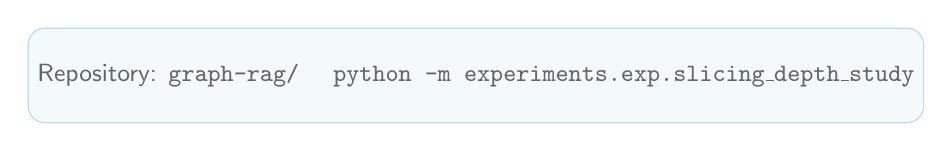
\begin{tikzpicture}
  \node[draw=c1!30,rounded corners=6pt,fill=c1!5,
        minimum width=9cm,minimum height=1.2cm,
        font=\small\sffamily\color{black!60},align=center]
    {Repository: \texttt{graph-rag/} \quad
     \texttt{python -m experiments.exp.slicing\_depth\_study}};
\end{tikzpicture}
\end{frame}

\end{document}
